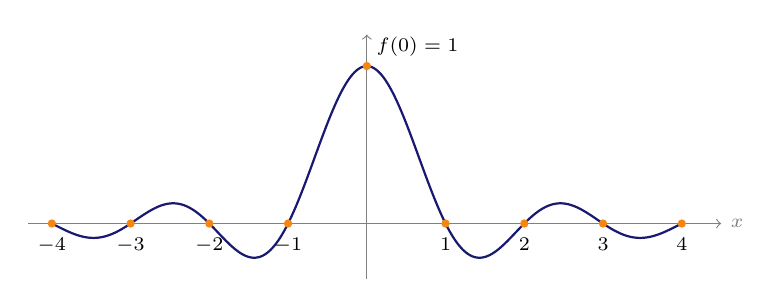
\begin{tikzpicture}[x=1cm,y=2cm,every node/.style={font=\scriptsize}]
\draw[->,gray] (-4.3,0)--(4.5,0) node[right] {$x$};
\draw[->,gray] (0,-.35)--(0,1.2);
\draw[MidnightBlue,thick,domain=-4:4,samples=401] plot (\x,{abs(\x)<0.00001 ? 1 : sin(180*\x)/(pi*\x)});
\foreach \k in {-4,-3,-2,-1,1,2,3,4}{\fill[BurntOrange] (\k,0) circle (1.5pt);\node[below] at (\k,-.03) {$\k$};}
\fill[BurntOrange] (0,1) circle (1.5pt);\node[above right] at (0,1) {$f(0)=1$};
\end{tikzpicture}
